%========
\section{Produit de convolution} 

\todoinline{Pour ajouter les ptés relatives aux transformées de Laplace et de Fourier, il faut le théorème de Fubini. On peut choisir de l'admettre.}

\begin{marginfigure}[0cm]
    \centering
    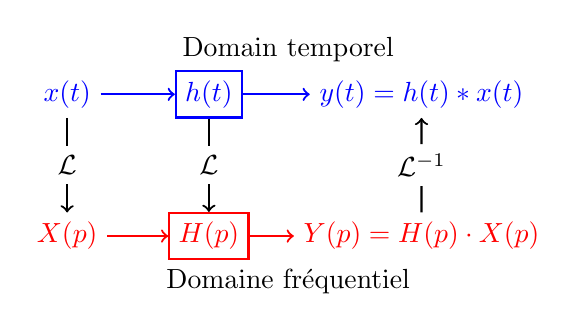
\begin{tikzpicture}

\begin{scope}[local bounding box=diagramme, scale=0.9, anchor=center, baseline]
    \node[blue] (x) at (0, 2) {$x(t)$};
    \node [draw, rectangle, thick, color=blue] (h) at (2, 2) {$h(t)$};
    \node[blue] (y) at (5, 2) {$y(t) = h(t) * x(t)$};
    \draw[->, thick, blue] (x) -- (h);
    \draw[->, thick, blue] (h) -- (y);
    
    \node (laplace1) at (0, 1) {$\mathcal{L}$};
    \node (laplace2) at (2, 1) {$\mathcal{L}$};
    \node (inverse_laplace) at (5, 1) {$\mathcal{L}^{-1}$};
    \draw[thick] (x) -- (laplace1);
    \draw[thick] (h) -- (laplace2);
    \draw[<-, thick] (y) -- (inverse_laplace);
    
    \node[red] (X) at (0, 0) {$X(p)$};
    \node [draw, rectangle, thick, color=red] (H) at (2, 0) {$H(p)$};
    \node[red] (Y) at (5, 0) {$Y(p) = H(p) \cdot X(p)$};
    \draw[->, thick, red] (X) -- (H);
    \draw[->, thick, red] (H) -- (Y);
    
    \draw[->, thick] (laplace1) -- (X);
    \draw[->, thick] (laplace2) -- (H);
    \draw[thick] (inverse_laplace) -- (Y);
\end{scope}
\node at (diagramme.north) [above] {Domain temporel};
\node at (diagramme.south) [below] {Domaine fréquentiel};
    
\end{tikzpicture}
    \caption{Source : \url{https://commons.wikimedia.org/wiki/File:Time_and_frequency_domains.svg?uselang=fr}}
\end{marginfigure}

\begin{defi}[Produit de convolution]
Soient $f$ et $g$ deux fonctions continues par morceaux sur $\R$. Pour tout $x \in \R$, on définit, lorsque l'intégrale converge,
\begin{equation}\label{defconvolution}
(f \ast g)(x) = \int_{\R} f(x-y) g(y) \d y.
\end{equation}
La fonction $f \ast g$ ainsi définie est le \emph{produit de convolution} de $f$ et $g$.
\end{defi}

\todoinline{Ajouter la source du concours : Maths 1 - Centrale Supélec 2012}

%-----------
\subsection{Propriétés du produit de convolution}

\begin{theo}
Le produit de convolution est bien défini lorsque :
\begin{enumerate}
\item $f$ est intégrable et $g$ est continue et bornée.

\item les fonctions $f$ et $g$ sont de carré intégrable.
\end{enumerate}
\end{theo}

\begin{demo}
\begin{enumerate}
\item On remarque que $\module{f(x - \cdot) g(\cdot)} \leq \norm{g}_\infty \module{f(x - \cdot)}$. Ainsi, la fonction $y \mapsto \module{f(x - \cdot) g(\cdot)}$ est dominée par une fonction intégrable, donc est intégrable.

\item On remarque que $\module{f(x - \cdot) g(\cdot)} \leq \frac{f(x - \cdots)^2 + g(\cdot)^2}{2}$. Ainsi, la fonction $y \mapsto \module{f(x - \cdot) g(\cdot)}$ est dominée par une fonction intégrable, donc est intégrable.
\end{enumerate}
\end{demo}

\begin{theo}
Si $f \ast g$ est bien défini, alors $f \ast g = g \ast f$.
\end{theo}

\begin{demo}
Il suffit d'effectuer le changement de variable affine $u = x - y$.
\end{demo}


\todoinline{Ajouter des hypothèses au théorème suivant ?}

\begin{theo}{}
\[
\mathcal{L}(f \ast g) = \mathcal{L}(f) \mathcal{L}(g)
\]
\end{theo}

%-----------
\subsection{Approximation de l'unité}

Pour tout entier naturel $n$, on note
\[
h_n : t \mapsto \frac{(1 - t^2)^n}{\lambda_n} \indicatrice{\interff{-1}{1}},
\]
où $\lambda_n = \displaystyle\int_{-1}^1 (1 - t^2)^n \d t$.

\begin{theo}
Pour tout $n$ entier naturel,
\begin{enumerate}
\item $h_n$ est positive sur $\R$ ;
\item $\int_{-\infty}^{+\infty} h_n(t) \d t = 1$ ;

\item $\forall\, \varepsilon > 0$, $\displaystyle\lim_{n\to+\infty} \int_{-\infty}^{-\varepsilon} h_n(t) \d t = 0$ et $\displaystyle\lim_{n\to+\infty} \int_{\varepsilon}^{+\infty} h_n(t) \d t = 0$.
\end{enumerate}
La suite $(h_n)$ est une \definir{approximation de l'unité}.

De plus, pour toute fonction $f$ continue bornée sur $\R$, $(f \ast h_n)_{n\in\N}$ converge simplement vers $f$ sur $\R$ 
\end{theo}

\begin{exercice}
Soit $f$ une fonction continue bornée et $n \in \N$.
\begin{questions}
\item Montrer que $h_n$ est positive sur $\R$ et que $\displaystyle\int_{-\infty}^{+\infty} h_n(t) \d t = 1$.

\item Montrer que $\lambda_n \geq \frac{1}{n + 1}$.
\end{questions}

Soit $\varepsilon > 0$.

\begin{questions}[resume]
\item Si $\module{\varepsilon} \geq 1$, calculer $\int_\varepsilon^{+\infty} h_n(t) \d t$ et $\int_{-\infty}^{-\varepsilon} h_n(t) \d t$.

\item Si $\module{\varepsilon} < 1$, montrer que $\int_\varepsilon^1 h_n(t) \d t \leq (n + 1) (1 - \varepsilon^2)^n$.

\item En déduire que $(h_n)$ est une approximation de l'unité.
\end{questions}

Soit $x \in \R$ et $\varepsilon > 0$.
\begin{questions}[resume]
\item Montrer qu'il existe $\delta > 0$ tel que
\[
\module{t} \leq \delta \, \Rightarrow\, \module{f(x - t) - f(x)} \leq \varepsilon.
\]

\item Montrer qu'il existe un réel $n_0$ tel que pour tout $n \geq n_0$,
\[
\int_{-\infty}^{-\delta} h_n(t) \d t \leq \varepsilon
\text{ et }
\int_{\delta}^{+\infty} h_n(t) \d t \leq \varepsilon.
\]

\item En déduire que $(f \ast h_n)$ converge simplement vers $f$ sur $\R$.
\end{questions}
\end{exercice}


\begin{demo}
\begin{questions}
\item Ces deux premiers points sont des conséquences de la définition de $h_n$.

\item Si $t \in [-1, 1]$, alors $t^2 \leq t$. Ainsi, d'après la définition,
\[
\lambda_n
= \int_{-1}^1 (1 - t^2)^n \d t
\geq \int_{-1}^1 (1 - t)^n \d t
= \frac{1}{n + 1}.
\]


\item Comme $h_n$ est nulle en dehors de $[-1, 1]$, alors 
\[
\int_\varepsilon^{+\infty} h_n(t) \d t
= \int_{-\infty}^{-\varepsilon} h_n(t) \d t
= 0.
\]

\item Si $0 \leq \varepsilon \leq t < 1$, alors $\varepsilon^2 \leq t^2$. Ainsi,
\[
\int_\varepsilon^1 h_n(t) \d t
\leq \int_\varepsilon^2 \frac{(1 - \varepsilon^2)^n}{\lambda_n} \d t
\leq (n + 1) (1 - \varepsilon^2)^n.
\]

De manière analogue, si $-1 \leq \varepsilon \leq 0$, alors
\[
\int_{-1}^{-\varepsilon} h_n(t) \d t \leq (n + 1) (1 - \varepsilon^2)^n.
\]

\item Finalement, d'après le théorème des croissances comparées,
\[
\forall \varepsilon > 0,\,
\displaystyle\lim_{n\to+\infty} \int_{-\infty}^{-\varepsilon} h_n(t) \d t
= \displaystyle\lim_{n\to+\infty} \int_{\varepsilon}^{+\infty} h_n(t) \d t
= 0.
\]

\item Comme $f$ est continue en $x$, il existe un réel $\delta$ tel que pour tout $t \in [-\delta, \delta]$,
\[
\module{f(x - t) - f(x)} \leq \varepsilon.
\]

\item Il suffit de traduire avec des quantificateurs la limite démontrée dans les questions précédentes.

\item On utilise la relation de Chasles ainsi que les questions précédentes, pour $n \geq n_0$, :
\begin{align*}
\module{(f \ast h_n)(x) - f(x)}
&= \module{\int_{-\infty}^{+\infty} f(x - t) h_n(t) \d t - f(x) \int_{-\infty}^{+\infty} h_n(t) \d t}\\
&\leq
\int_{-\infty}^{-\delta} \module{f(x - t) - f(t)} h_n(t) \d t
+ \int_{-\delta}^{\delta} \module{f(x - t) - f(t)} h_n(t) \d t
+ \int_{\delta}^{+\infty} \module{f(x - t) - f(t)} h_n(t) \d t\\
&\leq 2 \norm{f}_{\infty} \left(\int_{-\infty}^{-\delta} h_n(t) \d t + \int_{\delta}^{+\infty} h_n(t) \d t\right) + \varepsilon \int_{-\delta}^{\delta} h_n(t) \d t\\
&\leq 4 \norm{f}_{\infty} \varepsilon + \varepsilon \int_{-\delta}^{\delta} h_n(t) \d t\\
&\leq 4 \norm{f}_{\infty} \varepsilon + \varepsilon \int_{-\infty}^{+\infty} h_n(t) \d t\\\\
&\leq (4 \norm{f}_\infty + 1) \varepsilon.
\end{align*}
On obtient ainsi la convergence simple annoncée.
\end{questions}
\end{demo}